\clearpage
\section{Construir y emular}

Antes de continuar con las siguientes aplicaciones, y ya que tenemos lista nuestro primer desarrollo listo para ser usado, vamos ver como podemos  ejecutarlo en un emulador y en un terminal Android real, además de poder depurar el código desde el navegador Chrome como si de una página web se tratase. De esta forma podremos ver probar la aplicación sobre un terminal real de manera fácil y rápida.

Este método no tiene porque sustituir al servidor de desarrollo local que ejecutamos con \emph{ionic serve}. Este servidor se caracteriza por ser más rápido a la hora de testear pequeños cambios, en especial si estos afectan al diseño, y sobrecarga menos la máquina en la que lo ejecutemos que lo que lo hace un emulador. Aún así, resulta evidente la necesidad de probar las aplicaciones en los terminales objetivo. Una limitación muy importante que tiene ejecutar la aplicación sobre él servidor de desarrollo es la imposibilidad de emular las \glspl{API} de los dispositivos, por lo que si queremos hacer pruebas con los sensores, por ejemplo, el \gls{GPS}, necesitaremos utilizar un emulador o un dispositivo real. Por lo general, ambas formas son usadas a la hora de desarrollar la aplicación eligiendo una u otra según el cambio que queramos probar.

Por último tendremos que generar un ejecutable válido y reconocible por el sistema para poder distribuir nuestra aplicación. Explicaremos como hacer esto generando una \gls{APK} con la que poder instalar la aplicación en terminales Android.

Nos vamos a centrar en terminales con sistema operativo Android, debido a su popularidad, a que los recursos software necesarios son gratuitos y a que no requiere de un sistema operativo especial para poder desarrollar en él. Aún así, lo explicado en este capitulo es valido para otras plataformas siempre y cuando dispongamos de los recursos necesarios.

Antes de continuar, debemos asegurarnos de que tenemos instalado en nuestra máquina la suite de Android. Podemos ver una explicación de como instalar este software necesario en el anexo \nameref{ch:androidTools}. Aunque todas la acciones que veamos a continuación las hagamos a través de Ionic CLI, este necesita usar las herramientas que proporciona \emph{Google} para generar una aplicación nativa, que es la que realmente se ejecuta en los terminales. Además, el emulador que utilizaremos forma parte de esta suite.

\subsection{Añadir plataforma objetivo}

Lo primero que debemos hacer es añadir una plataforma objetivo a nuestro proyecto. Con esto configuramos nuestro proyecto indicando para que plataformas queremos que se generen los diferentes instaladores. En primer lugar vamos a ver que plataformas tenemos disponible en nuestro ordenador. Esto lo hacemos utilizando Ionic CLI dentro del directorio de nuestro proyecto.

\begin{figure}[H]
\centering
    \centering
        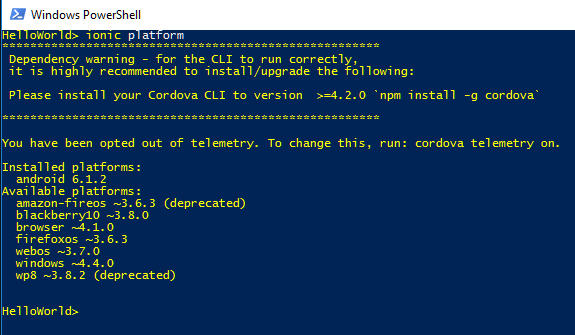
\includegraphics[width=0.8\textwidth]{Figures/ch2/BuildAndEmulate/available_platforms}
    \caption{Listado de plataformas disponibles para incluir en nuestro proyecto.}
\end{figure}

Como hemos dicho al inicio del capitulo, nos vamos a centrar en la plataforma Android, por lo que es la única que necesitamos añadir.

\begin{figure}[H]
\centering
    \centering
        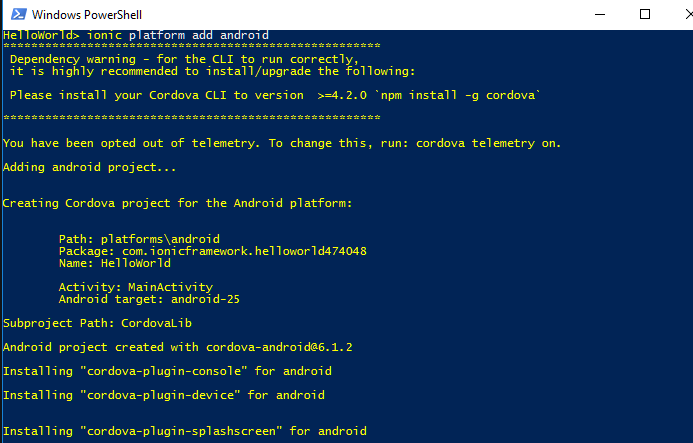
\includegraphics[width=0.8\textwidth]{Figures/ch2/BuildAndEmulate/add_android}
    \caption{Comando a ejecutar si queremos añadir la plataforma Android a la lista de plataformas objetivo de nuestra aplicación.}
\end{figure}

Con esto nuestro proyecto estaría preparado para ser ejecutado en un terminal o emulador Android, y para más tarde, generar el \gls{APK}.

\subsection{Emular aplicación}

Como se ha comentado, Ionic CLI nos permite arrancar un emulador Android en nuestra máquina de desarrollo y ejecutar sobre él la aplicación. Para ello utiliza Android Emulator, un emulador que ofrece Google como parte del \gls{SDK} de Android. Ionic se encarga, ejecutando un único comando, de compilar el proyecto, generar el instalable, arrancar el emulador e instalar en él nuestra aplicación. Un ejemplo del comando que hace todo esto es:

\begin{lstlisting}[language=bash]
  # ionic emulate android --target=Nexus5
\end{lstlisting}

Como vemos, en el comando debemos indicar sobre que plataforma queremos realizar la emulación. Como opción, podemos seleccionar que \gls{AVD} queremos utilizar, en caso de no indicarlo, Ionic CLI utilizará el primero que encuentre. Podemos encontrar más información sobre los \gls{AVD} en el anexo \nameref{ch:androidTools}, y más concretamente, en la sección \nameref{sec:AndroidEmulator}.

La ejecución de este comando iniciará una serie de tareas que podremos ir viendo aparecer en la consola. Justo antes de acabar (tarda unos segundos), se iniciará el emulador (si no estaba ya en ejecución) y a continuación, se iniciará la aplicación automáticamente en este.

\begin{figure}[H]
\centering
    \centering
        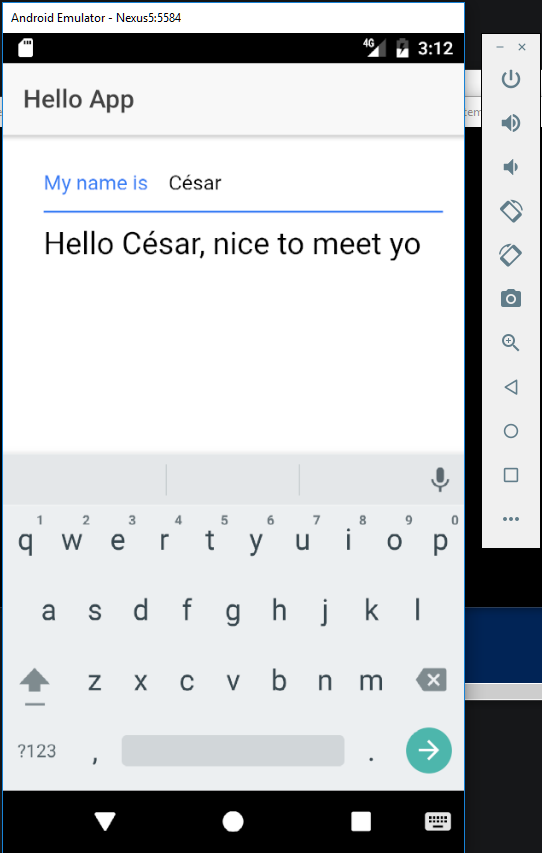
\includegraphics[width=0.4\textwidth]{Figures/ch2/BuildAndEmulate/landscape_emulator}
    \caption{Nuestra aplicación vista en el emulador.}
\end{figure}

\subsection{Depurar una aplicación que está siendo emulada}

Ya hemos dicho que durante la false de desarrollo, la mejor forma de probar y depurar nuestra aplicación es haciendo uso de la utilidad \emph{ionic serve} y de nuestro navegador favorito. Aún así, en ocasiones es necesario poder depurar la aplicación mientras se ejecuta en el emulador, por ejemplo, para probar el uso de determinados sensores, gestos sobre la pantalla que no podemos realizar en el navegador o simplemente comprobar que la aplicación se ve como debe en un terminal similar al emulado.

Para esto vamos a utilizar el navegador Chrome, que nos permite acceder a las aplicaciones que se ejecuten en el emulador o terminal conectado que usen tecnología web. Aunque aquí nos centramos en aplicaciones híbridas, podemos usar también este mismo método para aplicaciones que se estén ejecutando en el navegador del dispositivo. Vamos a emular la aplicación del mismo modo que hicimos anteriormente:

\begin{lstlisting}[language=bash]
  # ionic emulate android --livereload --target=Nexus5
\end{lstlisting}

Añadiendo \emph{--livereload} conseguimos algunas de las facilidades que tenemos al utilizar \emph{ionic serve}:

\begin{enumerate}
  \item Ver los cambios realizado en el código de manera inmediata sin necesidad de tener que volver a lanzar el comando para que vuelva a compilar la aplicación y la vuelva a ejecutar.
  \item Poder depurar el código sin que este esté compilado.
\end{enumerate}

\warningbox{En el momento de escribir este documento, la opción \emph{--livereload} se encuentra en fase \emph{beta}, por lo que puede no funcionar correctamente. De ser así, nos veremos obligados a usar el método manual y recompilar la aplicación cada vez que efectuemos un cambio.}

Una vez que la aplicación se esté ejecutando, iniciamos el \emph{Chrome} y abrimos la consola para desarrolladores (desde las opciones de Chrome > Más herramientas > Herramientas de desarrolladores, o pulsando F12, o pulsando ctrl + shift + I). Dentro de la consola, en opciones > \emph{More tools} seleccionamos \emph{Remote Devices}.

\begin{figure}[H]
\centering
    \centering
        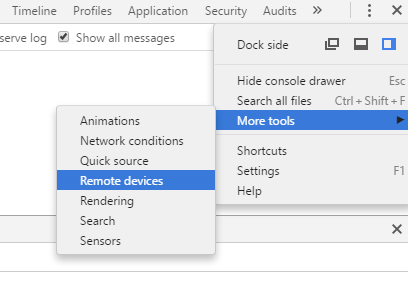
\includegraphics{Figures/ch2/BuildAndEmulate/how_open_remote_devices}
    \caption{Opción para abrir la ventana de dispositivos remotos.}
\end{figure}

Esto nos abrirá una ventana dentro de la consola donde aparecerán todos los dispositivos que tengamos conectados (emuladores, terminales conectados al PC, incluso los Chromecast si disponemos de alguno en nuestra red). En esta lista de dispositivos encontraremos nuestro emulador, en él, aparecerá nuestra aplicación, la cual podremos \emph{Inspeccionar}.

\begin{figure}[H]
\centering
    \centering
        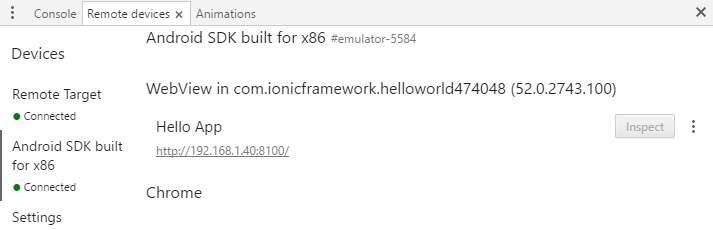
\includegraphics[width=0.8\textwidth]{Figures/ch2/BuildAndEmulate/remote_devices_list}
    \caption{Lista de dispositivos disponibles para depurar. Entre ellos se encuentra nuestro emulador con nuestra aplicación híbrida abierta.}
\end{figure}

Si seleccionamos la opción inspeccionar, se nos abrirá una ventana del navegador en la que veremos lo mismo que se esta viendo en esos momentos en el emulador. Podremos ver el detalle de los elementos del \gls{HTML} de la misma manera que si fuera una página web corriente abierta directamente en el navegador. Además, podremos controlar la aplicación desde el navegador, así, cualquier acción que llevemos a cabo, como pulsar algún elemento, escribir, arrastar con el botón del ratón pulsado, \ldots  se verá reflejado también en el navegador.

Podremos acceder a los ficheros \emph{.ts} y poner puntos de ruptura donde nos interese detener la ejecución del código. Como se comentaba anteriormente, esta posibilidad solo se da con la opción \emph{--livereload}. De no ser así, tendremos que buscar el trozo de código que nos interesa en el fichero ya compilado.

\begin{figure}[H]
\centering
    \centering
        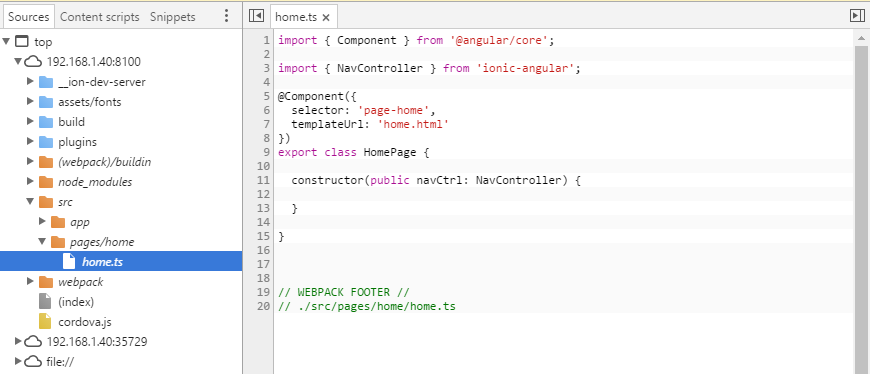
\includegraphics[width=\textwidth]{Figures/ch2/BuildAndEmulate/livereload_code_dev_tool}
        \hfill \break
        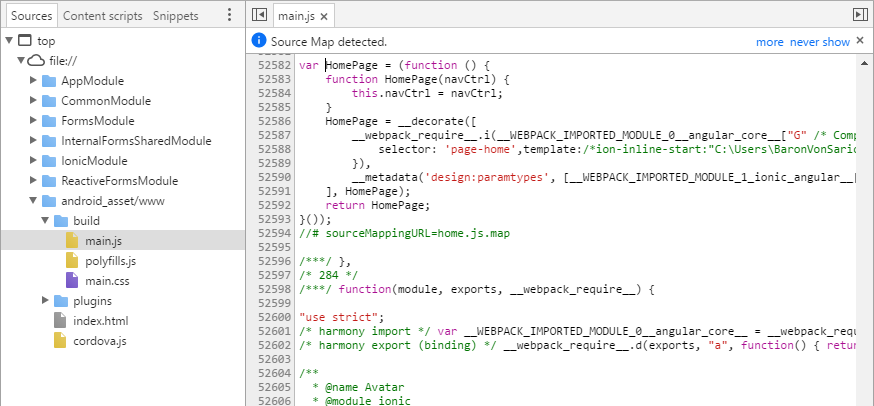
\includegraphics[width=\textwidth]{Figures/ch2/BuildAndEmulate/nolivereload_code_dev_tool}
    \caption{Diferencia entre como se ve el código sin compilar, emulado con la opción \emph{--livereload} (arriba), y el código compilado (abajo).}
\end{figure}

Podemos probar a cambiar el código y ver como la aplicación se recarga nada más guardamos el cambio. Por ejemplo, vamos a hacer que se escriba una entrada en el log al iniciar la aplicación. Abrimos el fichero \emph{home.ts} de nuestra página y editamos el constructor de la siguiente manera:

{\begin{lstlisting}[style=htmlcssjs,frame=tlrb,xleftmargin={0.2cm}]
constructor(public navCtrl: NavController) {
    console.log("HelloWorld application is running."):
  }

\end{lstlisting}}

Una vez que la aplicación haya terminado de recargar, apenas tarda unos segundos, podremos comprobar que el cambio en efecto se ha efectuado y ver en la consola el mensaje anterior.

\begin{figure}[H]
\centering
    \centering
        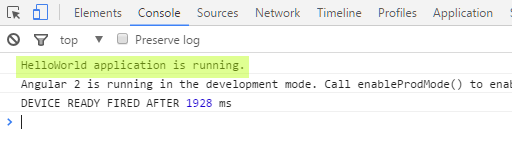
\includegraphics[width=0.8\textwidth]{Figures/ch2/BuildAndEmulate/state_log}
    \caption{La aplicación muestra por consola el mensaje de inicio.}
\end{figure}

También podremos hacer el cambio sobre el script que se está ejecutando sobre el mismo navegador y guardar el cambio utilizando la combinación ctrl + s. Este cambio solo será temporal y hasta que se vuelva a recargar el fichero JavaScript, pero será válido siempre que el flujo de ejecución pase por él. Tampoco modifica el código sobre el que estamos trabajando, ya que el cambio se guarda en la versión del script que utiliza el navegador.

\subsection{Ejecutar una aplicación en un terminal conectado} \label{subsec:runInDevice}

Si disponemos de uno o varios terminales en los que poder probar la aplicación, podemos conectarlos a nuestro ordenador y hacer que ejecute el código del mismo modo que ocurre en el emulador teniendo también la opción de depuración desde Chrome.

En primer lugar, debemos tener el terminal conectado al ordenador, y asegurarnos de tener todos los drivers instalados. Además, debemos de habilitar el modo \emph{debug} vía \gls{USB} en el móvil y autenticar nuestro PC en el móvil. En la web de desarrolladores de Google nos explican como poder hacer esto \emph{https://developers.google.com/web/tools/chrome-devtools/remote-debugging/}.

Cuando tengamos nuestro terminal listo, llegará el momento de ver nuestra aplicación en él. Como podremos imaginar, esto se consigue utilizando Ionic CLI:

\begin{lstlisting}[language=bash]
  # ionic run android --livereload
\end{lstlisting}

Y listo. Si todo va bien, al cabo de unos segundos debería aparecer nuestra aplicación en el terminal.

Al igual que ocurría con el emulador, podremos depurar nuestra aplicación utilizando el navegador Chrome, siguiendo los mismos pasos explicados anteriormente, pero seleccionando nuestro terminal en la lista de dispositivos.

\begin{figure}[H]
\centering
    \centering
        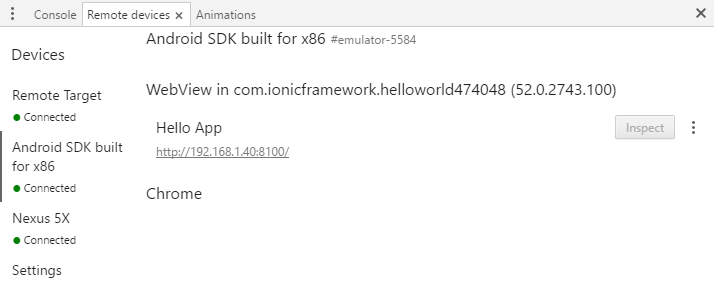
\includegraphics[width=0.8\textwidth]{Figures/ch2/BuildAndEmulate/remote_devices_list_nexus5}
    \caption{El terminal Android conectado a nuestro equipo aparece listado entre los dispositivos disponibles en Chrome.}
\end{figure}

Esta operación nos dejaría la aplicación instalada en nuestro terminal, por lo que al desconectar el dispositivo del ordenador podríamos seguir usandola como si de otra aplicación se tratase (algo útil si necesitamos hacer pruebas con el \gls{GPS}).

\subsection{Generar el instalador. El APK.}

Cuando ya demos por buena nuestra aplicación, o simplemente queramos compartirla con alguien sin tener que compartir el código y haciendo que sea él quien lo compile, será el momento de generar el instalador para las diferentes plataformas. Como estamos trabajando para la plataforma Android, en nuestro caso generaremos un fichero \emph{.apk}. Este fichero podremos compartirlo con cualquier usuario de Android y podrá instalarlo en su dispositivo. También podrá ser subido a la tienda de aplicaciones de Android, \emph{Play Store}, para que pueda ser descargado por cualquier usuario. Para esto último, será necesario firmar el \gls{APK}.

Antes de esto, vamos a darle un último toque de personalización a nuestra aplicación. Si ya hemos ejecutado la aplicación en el terminal como se explicaba en el apartado anterior, nos habremos fijado en dos detalles. Por un lado, el icono que aparece en nuestro dispositivo representando a nuestra aplicación es el icono de Apache Cordova. Con el splash, la pantalla que aparece al iniciar la aplicación, ocurre lo mismo. Ambos son generados y configurados por defecto al añadir una nueva plataforma al proyecto.

Para poder personalizar tanto el icono como el splash, necesitamos de una imagen para cada uno de ellos en formato \emph{.png, .psd o .ai}. Ambas tendrán que tener el elemento principal de la imagen debe estar centrado, ya que Ionic recortará la imagen para ajustarla a diferentes tamaños de pantalla. En cuanto al tamaño, el icono tendrá que tener un tamaño mínimo de 192x192 píxeles y no tendrá que tener los bordes redondeados ya que este efecto lo aplica la propia plataforma. El splash, deberá medir un mínimo de 2208x2208 píxeles.

Una vez creadas las imágenes, tendremos que colocarlas dentro de nuestro proyecto en la capeta \emph{resources} con los nombres \emph{icon.png y splash.png} (o con la extensión del formato que hayamos elegido). Ejecutamos de nuevo un comando proporcionado por Ionic CLI el cual generará, a partir de nuestras imágenes, diferentes iconos y splash para los diferentes dispositivos y los dejará preparados para cuando se genere el instalador.

\begin{lstlisting}[language=bash]
  # ionic resources
\end{lstlisting}

\notebox{El comando \emph{ionic resources} dispone de dos opciones, \emph{--icon y --splash}, por si solo queremos generar uno de los dos elementos.}

Para más información, podemos consultar la documentación que proporciona Ionic en su primera versión, pero que también es aplicable para la versión 2 en  \url{http://ionicframework.com/docs/cli/icon-splashscreen.html}.

Ya con todo listo, podemos generar nuestro APK. Ejecutamos el siguiente comando:

\begin{lstlisting}[language=bash]
  # ionic build android
\end{lstlisting}

Al finalizar, aparecerá la ruta donde se encuentra el APK. Lo renombramos con un nombre que nos resulte identificable y ya podemos probar a instalarlo en cualquier dispositivo Android.

\warningbox{En caso de tener ya la aplicación instalada por otro método, por ejemplo el explicado en el punto \nameref{subsec:runInDevice}, es posible que no podamos instalar la aplicación y recibamos un error a cambio. En este caso, es mejor desinstalar la aplicación y probar de nuevo. Lo mismo puede ocurrir si intentamos la misma operación pero en orden inverso.

Esto ocurre debido a que el nombre de la aplicación que usa Android internamente para identificarla es el mismo, pero la fuente de instalación son diferentes, por lo que pueden entrar en conflicto.}
